%-----------------------------------------------------------------
%	BASIC DOCUMENT LAYOUT
%-----------------------------------------------------------------
\documentclass{beamer}

% \usepackage[scaled]{helvet}
% \renewcommand\familydefault{\sfdefault}
\usefonttheme[onlymath]{serif}

\usepackage[T1]{fontenc}
\usepackage[utf8]{inputenc}
\usepackage{microtype}
\usepackage[british]{babel}
\usepackage{url}
\usepackage{ru-theme}

\usepackage[backend=bibtex, style=trad-abbrv, sorting=none, maxbibnames=3, maxcitenames=2]{biblatex}
\addbibresource{bibliography.bib}
\makeatletter
	\def\blx@maxline{77}
\makeatother

\usepackage{array}
\usepackage{multirow}

%-----------------------------------------------------------------
%	LISTINGS
%-----------------------------------------------------------------
\makeatletter

\newcount\bt@rangea
\newcount\bt@rangeb

\newcommand\btIfInRange[2]{%
    \global\let\bt@inrange\@secondoftwo%
    \edef\bt@rangelist{#2}%
    \foreach \range in \bt@rangelist {%
        \afterassignment\bt@getrangeb%
        \bt@rangea=0\range\relax%
        \pgfmathtruncatemacro\result{ ( #1 >= \bt@rangea) && (#1 <= \bt@rangeb) }%
        \ifnum\result=1\relax%
            \breakforeach%
            \global\let\bt@inrange\@firstoftwo%
        \fi%
    }%
    \bt@inrange%
}
\newcommand\bt@getrangeb{%
    \@ifnextchar\relax%
        {\bt@rangeb=\bt@rangea}%
        {\@getrangeb}%
}
\def\@getrangeb-#1\relax{%
    \ifx\relax#1\relax%
        \bt@rangeb=100000%   \maxdimen is too large for pgfmath
    \else%
        \bt@rangeb=#1\relax%
    \fi%
}

\newcommand<>{\btLstHL}[1]{%
  \only#2{\btIfInRange{\value{lstnumber}}{#1}{\color{orange!30}\def\lst@linebgrdcmd{\color@block}}{\def\lst@linebgrdcmd####1####2####3{}}}%
}%
\makeatother

\makeatletter
\newenvironment{btHighlight}[1][]
{\begingroup\tikzset{bt@Highlight@par/.style={#1}}\begin{lrbox}{\@tempboxa}}
{\end{lrbox}\bt@HL@box[bt@Highlight@par]{\@tempboxa}\endgroup}

\newcommand\btHL[1][]{%
  \begin{btHighlight}[#1]\bgroup\aftergroup\bt@HL@endenv%
}
\def\bt@HL@endenv{%
  \end{btHighlight}%
  \egroup
}
\newcommand{\bt@HL@box}[2][]{%
  \tikz[#1]{%
    \pgfpathrectangle{\pgfpoint{1pt}{0pt}}{\pgfpoint{\wd #2}{\ht #2}}%
    \pgfusepath{use as bounding box}%
    \node[anchor=base west, fill=orange!30,outer sep=0pt,inner xsep=1pt, inner ysep=0pt, rounded corners=3pt, minimum height=\ht\strutbox+1pt,#1]{\raisebox{1pt}{\strut}\strut\usebox{#2}};
  }%
}
\makeatother

\usepackage[formats]{listings}
\usepackage{relsize}
% \usepackage{chngcntr}
\usepackage{lstlinebgrd}

\definecolor{keywords}{HTML}{268bd2}
\definecolor{background}{HTML}{eee8d5}
\definecolor{comments}{HTML}{586e75}

\lstloadlanguages{C++}
% \lstset{language=C++,
% 		basicstyle=\smaller\ttfamily,
% 		% keywordstyle=\bfseries,
% 		% morecomment=[l][\color{magenta}]{\#},
% 		keywordstyle=\color{keywords},
% 		commentstyle=\color{comments}\itshape,
% 		% backgroundcolor=\color{background},
% 		frame=tb,
% 		tabsize=2,
% 		breaklines=true,
% 		breakatwhitespace=true,
% 		numbers=left,
% 		numberstyle=\tiny,
% 		num
% 		bersep=7.5pt,
% 		moredelim=**[is][{\btHL[fill=blue!30,draw=blue,dashed,thin]}]{£}{£},
% 		moredelim=**[is][{\btHL[fill=red!30,draw=red,dashed,thin]}]{@}{@},
% 		moredelim=**[is][{\btHL[fill=green!30,draw=green,dashed,thin]}]{&}{&},
% 		xleftmargin=3ex}
\lstset{escapeinside={(*}{*)}}

\newcommand*{\inline}{\lstinline[basicstyle=\normalsize\ttfamily]}

%-----------------------------------------------------------------
%	MATHS AND SCIENCE
%-----------------------------------------------------------------
\usepackage{amsmath,amsfonts,amsthm,amssymb}
\usepackage{xfrac}
\usepackage[a]{esvect}
\usepackage{chemformula}
\usepackage{graphicx}

\usepackage[arrowdel]{physics}
	\renewcommand{\vnabla}{\vec{\nabla}}
	\renewcommand{\vectorarrow}[1]{\vec{#1}}
	\renewcommand{\vectorunit}[1]{\hat{#1}}
	\renewcommand*{\grad}[1]{\vnabla #1}
	\renewcommand*{\div}[1]{\vnabla \vdot \va{#1}}
	\renewcommand*{\curl}[1]{\vnabla \cp \va{#1}}
	\let\rot\curl

% SI units
\usepackage[separate-uncertainty=true]{siunitx}
\sisetup{range-phrase = \text{--}, range-units = single}
\DeclareSIPrePower\quartic{4}

%-----------------------------------------------------------------
%	PDF INFO AND HYPERREF
%-----------------------------------------------------------------
\usepackage{hyperref}
% \hypersetup{colorlinks, citecolor=black, filecolor=black, linkcolor=black, urlcolor=black}
\usepackage{cleveref}
	\crefname{section}{\S}{\SS}
	\Crefname{section}{\S}{\SS}
	\crefname{listing}{snippet}{}

\newcommand*{\mytitle}{Control of a Trailer}
\newcommand*{\myshorttitle}{Control of a Trailer}
\newcommand*{\mysubtitle}{How to steer a car when parking}
\newcommand*{\myauthor}{Alfredo Hernández}
\newcommand*{\myauthora}{David Masip}
\newcommand*{\myauthorb}{Martí Municoy}
\newcommand*{\myauthorc}{Jan-Hendrick Niemann}
\newcommand*{\myuni}{Universitat Autònoma de Barcelona}
\newcommand*{\mydegree}{Modelling for Science and Engineering}
\newcommand*{\mydate}{2nd February 2018}

\pdfstringdefDisableCommands{\def\and{and }}

\usepackage{hyperxmp}
% \hypersetup{pdfauthor={\myauthor}, pdftitle={\mytitle: \mysubtitle}}
\hypersetup{pdfauthor={\myauthor}, pdftitle={\mytitle}}

%-----------------------------------------------------------------
%	TITLE SECTION AND DOCUMENT BEGINNING
%-----------------------------------------------------------------

\title[\mytitle]{\mytitle}

\subtitle{\mysubtitle}

\author[Team 7]{ \myauthor \and \myauthora \and \myauthorb \and \myauthorc }% \and \myauthora \and \myauthorb \and \myauthorc}

% \institute[]{\myuni { --} \mydegree}
\institute[]{\mydegree}

\date[\mydate]{\mydate}

\hypersetup{pdfauthor={\myauthor}, pdftitle={\mytitle: \mysubtitle}}

\begin{document}

\begin{frame}
	\titlepage
\end{frame}

%-----------------------------------------------------------------
%	DOCUMENT BODY
%-----------------------------------------------------------------
\section{Introduction}
\begin{frame}{Introduction}
	% \tableofcontents
	\begin{itemize}
		\item Theoretical Physics and Pure Mathematics in the old-fashioned sense are almost platonic.
		\item Programming is a must-have skill in all fields.
		\item An example of the challenges introduced by programming.
		\item Real life examples of programming in the academic and professional world.
	\end{itemize}
\end{frame}

%-----------------------------------------------------------------
% \section{A change of mindset}
% \begin{frame}[fragile]{A change of mindset}
% \begin{onlyenv}<+->
% \begin{onlyenv}<1-2>{\Large An simple example \medskip}\end{onlyenv}

% \begin{onlyenv}<1>
% \begin{lstlisting}
% // Initialize membrane potential matrix
% vector< vector<double> > v;
% v.resize(steps, vector<double>(neurons));
% // Initialise v
% for (int n = 0; n < neurons; n++) {
% 	v[0][n] = v0;
% }
% \end{lstlisting}
% \end{onlyenv}

% \begin{onlyenv}<2>
% \begin{lstlisting}
% // Initialize membrane potential matrix
% vector< vector<double> > v;
% v.resize(£steps£, vector<double>(£neurons£));
% // Initialise v
% for (int n = 0; n < neurons; n++) {
% 	v[0][n] = v0;
% }
% \end{lstlisting}
% \begin{tabular}{ll}
% 	& \multirow{2}{*}{
\includegraphics[scale=0.4]{images/emote} } \\
% 	\inline|v| matrix of $\sim\num{e10}$ \inline|double| elements (\inline|steps| $\times$ \inline|neurons|) \\
% 	$\quad \Rightarrow$ \SI{10}{GB} of RAM + hours of compile time \\
% \end{tabular}
% \end{onlyenv}

% \begin{onlyenv}<3>
% {\Large Bad \medskip}
% \begin{lstlisting}
% // Initialise membrane potential matrix
% vector< vector<double> > v;
% v.resize(@steps@, vector<double>(neurons));
% \end{lstlisting}

% {\Large Good \medskip}
% \begin{lstlisting}
% // Initialise membrane potential matrix
% vector< vector<double> > v;
% v.resize(&2&, vector<double>(neurons));
% \end{lstlisting}
% \end{onlyenv}

% \begin{onlyenv}<4>
% \begin{onlyenv}<4>{\Large Implementation \medskip}\end{onlyenv}

% Euler method calculations inside a loop:
% \begin{lstlisting}[firstnumber=7]
% v[1][n] = v[0][n] + h * ( pow(v[0][n], 2) + I[i-1] + eta[n] + J * syn_act[i-1] );
% \end{lstlisting}

% The useful data is directly saved into a text file on a loop, and the two vectors \inline|v[0][n]| and \inline|v[1][n]| are recycled.
% \begin{lstlisting}[firstnumber=24, linebackgroundcolor={%
% 	\btLstHL<4>{25	,28}%
% 	}]
% 		v_avg[i] += v[1][n];
% 		v[0][n] = v[1][n]; // Reset matrix
% 	}
% 	// Save values on files
% 	v_file << v_avg[i]/neurons << ", " ;
% \end{lstlisting}
% The program now uses only a couple \si{MB} of RAM, and it compiles in a matter of minutes.
% \end{onlyenv}

% \end{onlyenv}

% \end{frame}

% %-----------------------------------------------------------------
% \section{Just another tool}
% \begin{frame}{Just another tool}
% 	\begin{figure}[H]
% 		\centering
% 		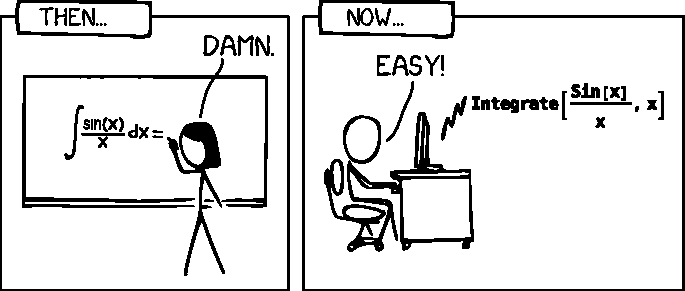
\includegraphics[scale=0.8]{images/xkcd}
% 		\label{fig:xkcd}
% 	\end{figure}
% \end{frame}

% %-----------------------------------------------------------------
% % \section{Programming IRL}
% \begin{frame}{Programming IRL}
% \begin{onlyenv}<1-3>

% 	\begin{itemize}[<+->]
% 		\item \textbf{CRM} -- Computational Neuroscience, Complex Systems, ...
% 		\item \textbf{IFAE} -- PAU (Physics of the Accelerating Universe) \url{www.pausurvey.org/}
% 		\item \textbf{CERN} -- CERN Data Centre \url{home.cern/about/computing}
% 	\end{itemize}
% 	\begin{onlyenv}<2>
% 		\begin{figure}[H]
% 			\centering
% 			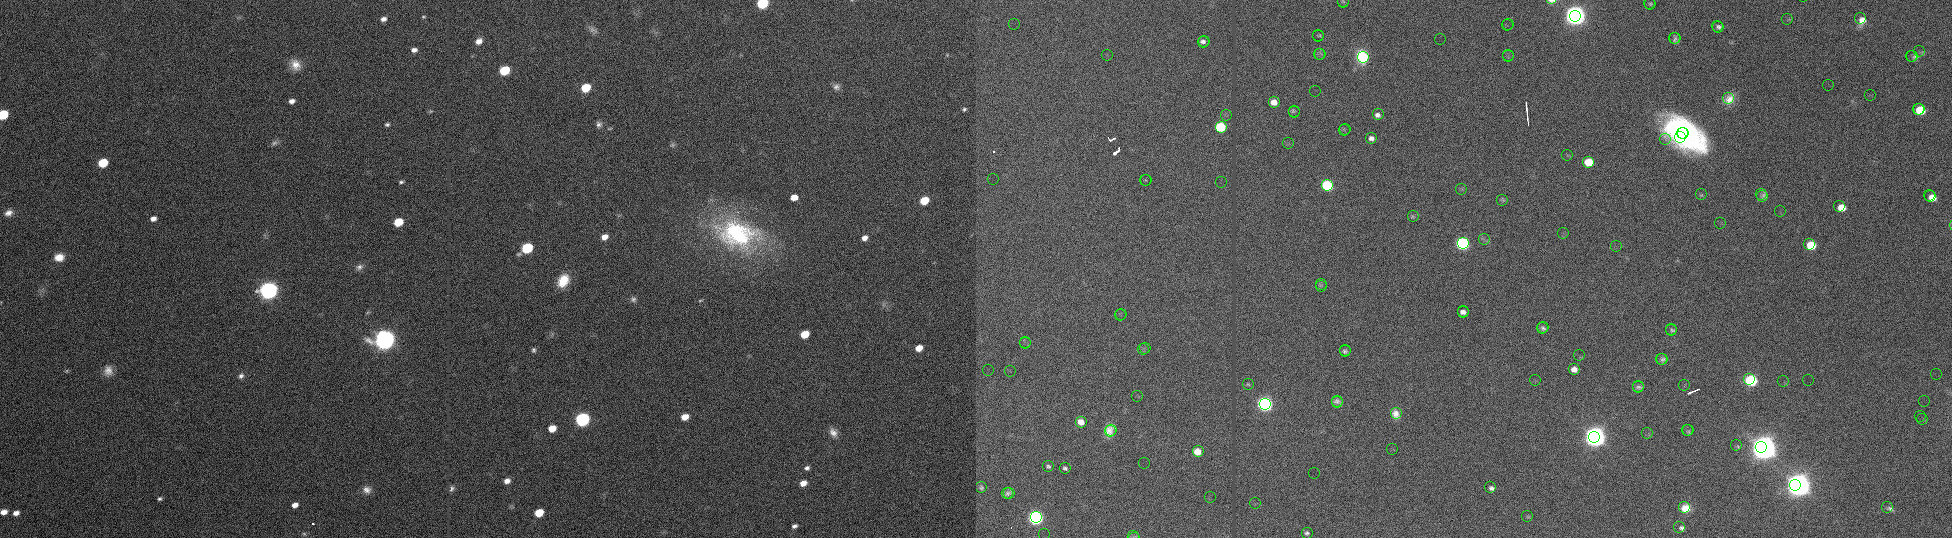
\includegraphics[scale=0.16]{images/pau-data}
% 			\caption{Automatised data processing}
% 			\label{fig:pau-data}
% 		\end{figure}
% 	\end{onlyenv}
% \end{onlyenv}

% \begin{onlyenv}<4>
% 	\begin{itemize}
% 		\item \textbf{IBM} -- IBM Watson \url{www.ibm.com/watson/}
% 		\item \textbf{Google} -- Research at Google \url{research.google.com/}
% 	\end{itemize}
% \end{onlyenv}

% %-----------------------------------------------------------------
% \begin{onlyenv}<5-6>
% {\Large Google Research Europe}

% \begin{itemize}
% 	\item <5-6> \textbf{Statistical Learning \& Neural Networks}
% 	\begin{itemize}[<.->]
% 		\item Machine Learning
% 		\item Natural Language Understanding
% 		\item Machine Perception
% 	\end{itemize}
% 	\item <6> \textbf{Classical Information Theory}
% 	\begin{itemize}[<.->]
% 		\item Data Compression
% 	\end{itemize}
% \end{itemize}
% \end{onlyenv}

% \end{frame}

%-----------------------------------------------------------------
\end{document}

